% Main report .tex code to compile
\documentclass[10pt,a4paper]{article}
\usepackage{graphicx}
\usepackage{a4}
%\usepackage{fullpage}
\usepackage{url}
\usepackage[utf8]{inputenc}
\usepackage{amssymb}

\usepackage{graphicx}
\usepackage{epstopdf}
\usepackage[utf8]{inputenc}
\usepackage{amsmath}
\usepackage{amsfonts}
\usepackage[english]{babel}

\usepackage{listings}

\urldef{\mailsa}\path|bao-hoai.lam@univ-brest.fr,|
\urldef{\mailsc}\path|pottier@univ-brest.fr|    

\textwidth 16cm
\title{Toward networked automatic coastal observatories:\\
architecture and  applications of vision sensors\\ 
{\sl extended abstract}}

\author{{ \textbf{Bao Hoai Lam \dag},  \textbf{Bernard Pottier}} \\
\textit{Universit{\'e} de Brest, Lab-STICC, France}\\
\textit{\dag Cantho University, Vietnam}\\
bao-hoai.lam@univ-brest.fr, pottier@univ-brest.fr}
%

% (feature abused for this document to repeat the title also on left hand pages)

% the affiliations are given next; don't give your e-mail address
% unless you accept that it will be published



\begin{document}
\maketitle

%SECTION 1.2

 We describe principles and applications of a small environment sensing station with emphasis on 
vision analysis. Such cameras can be used to monitor coastal ecology, from insects, birds to fish or vessels. 
Local processing is done in the station using a parallel architecture as an accelerator to 
produce local diagnostics and avoid transmitting  huge amount of data to remote centers. 
High performance computing methodologies also allow to obtain flexibility for counting, tracking, classifying
mobile objects of different kinds..


\section {Application fields in wild life and environment}
\subsection {Context description}

Automatic observation of living species is on the agenda for several reasons. First, there are fears for effects of climate change for several genus, and it is important to understand evolution of the situation related to species and environment. Second, there is a significant development of genus without predators which unbalance some environments. For example, insect pests cause extensive damage in several tropical countries: brown planthoppers in Vietnam, or locusts in Africa.

Building automatic observatory can be of great help for knowledge and risks managements. This paper explains some technical difficulties and their potential solutions, with a special focus on vision systems oriented to diagnostics. The general orientation are set of  programmable small autonomous communicating systems than can 
do these {\sl local diagnostic}  and emit synthetic information toward remote databases.

We will start by explanations about several application fields that we plan to investigate.

\subsection {Application fields}
\subsubsection {Insect monitoring}
Research is active on subjects such as statistical counting of insects in flights \cite{Hart:2012:CIF:2425836.2425891}, or tracking moving insects \cite{Bee1247421} moving in 3D for over few second, or tracking and analyzing behaviors of insect colonies \cite{Balch:2001:ATA:375735.376434}. These works use cameras to track mobile insects in real time to better understand their behaviors and to help to model them as well.

High speed cameras \cite{BeeFrequency} have been used to capture honey bees in flight at 6,000 frames per second at the resolution 512x512. It was observed that the aerodynamics of honeybee flight are determined by low stroke amplitude ($~90^{o}$) and high wingbeat frequency ($~$230 Hz). This work  suggests that the peculiar kinematics of bees may reflect some special features of their flight muscles.

\subsubsection {Bird monitoring}

Seabirds and marine environment health have a close relationship since sea bird population changes are the result of climate changes, pollution, low breeding rates. To better understand ecosystem, the project 'Monitoring nesting seabirds' \cite{Seabird1} in West Wales was carried out in order to estimate the position of birds nesting on a cliff-face using computer vision approach. The project provides automatic tools to monitor widelife, especially Skomer Guillemots and other seabirds, so that clearer and more reliable information of nesting bird is collected for decision making. 

One of contributions of this project is  to classify flying birds automatically \cite{Atanbori2015}. This work allows extracting from appearance features to motion features of observed birds. In addition, normal Bayes network and Support Vector Machine (SVM) methods are used to classified bird features. Experiment shows that the classification time is around 20ms, which is suitable for real time applications.

Nevertheless, this work seems not to take into account some factors. First, it does not consider the feature extraction time which may consume much more time than the classification phase. Besides, the overall time for processing an image frame is not mentioned as well. This overall time is important because it can help to estimate the average frame rate to better measure the execution time of the system.

A bird image dataset is constructed to be a premise of automatic bird detection classification \cite{Naemura7351607} for ecological investigations. In the dataset, 32,000 individuals are annotated by using a still camera with a telephoto setup in which the average size of birds in the image is around 25 pixels. From this work, some machine learning algorithms can be applied in order to classify bird species.

\subsubsection {Underwater monitoring}

Cameras can be put underwater to follow fish behaviors and trajectories \cite{Beyan2016}. The idea is to help marine specialists 
to detect environmental changes deduced from the unusual trajectories of fish. 
Although there are  challenges of underwater environments and trajectory data,  this work proposes a method, which provide better results than state of art methods, to detect unusual fish trajectories.

A system to track multiple fish \cite{Underwater6898002} is proposed to confront with low-contrast and low-frame-rate underwater stereo cameras. This system uses histogram back projection approach on double local-thresholded images to segment fish shape accurately. Due to the low frame rate of cameras, a modified multiple-target Viterbi data association is used to deal with poor motion continuity and frequent entrance/exit of the field of view for fish targets. The proposed system gets 88\% success rate in term of fish tracking in low conditions and gives 6\% of mean absolute percentage error in fish length measurement under the low-contrast environment.  

\subsubsection {Plants observation}

In \cite{Ryu2012116}, an approach  to quantify the tree leaf area index (LAI) at ecosystem scale using upward pointing cameras is proposed. It was applied to oak-savanna ecosystem in California to identify phenological and abnormal events and to estimate seasonal to interannual variability of tree LAI at ecosystem. Upward pointing cameras are used instead of other devices since they are inexpensive, fast and accurate in monitoring ecosystem under forest canopies. In addition, they are able to validate LiDAR derived gap fraction and to match fields between LiDAR and photos taken from cameras.

An hyperspectral camera analyzes the spectrum of plant leaves to identify the plant water stress \cite{Hyperspectra001}. It helps automating on-the-go  mapping of plant stress so that people can intervene and ease problems before exceeding critical threshold. Experimental results indicate that this solution can help decision making for plant stress detection and management.


\subsubsection {Boat monitoring}

An imaging method \cite{Broggi2009} to detect the speed and other information of boats moving on a wide surface using a single camera was proposed in Venice to notify boat drivers the speed of their boats created. The truth is that vessels and motor boats cross the channels too fast and generate huge sea waves which erode the city's docks. That causes a lot of damage to the city and its ecosystem. From the data collection of the operation of this system during 2 continuous years, it is observed that speeds of vessels are in the controllable level in the monitoring area of the camera.

This solution can be realized using radar data analysis \cite{Radar4653898} but it is much more expensive. Moreover, it is difficult to recognize small boats with radar based techniques since their spectrum is similar to the wave's spectrum.

\section{Sensing station proposal}

A sensing station can be built from following components:

\begin{itemize}
\item Autonomous system node. An autonomous sensor \cite{Auto5475165} is a device that is generally able to perform its task without being connected to a control  unit. The emergence of application fields requires the increase of computational capabilities with suitable power consumption in the sensor node. Raspberry pi \cite{PI3}, NVIDIA Jetson Tk1 \cite{Jetson} are examples of such devices that are able to deal with new challenges of application fields (table \ref{img:PiJetson}). 

\begin{figure}[ht]
\centering
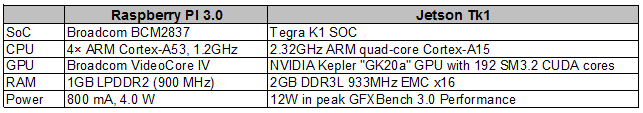
\includegraphics[width=3.0in,height=0.8in]{img/PiJetson.png}
\caption{Raspberry Pi 3.0 and NVIDIA Jetson Tk1 specifications.}
\label{img:PiJetson}
\end{figure}

\item Radio link and network organization. Sensor nodes connected each other mostly using radio connection in a network topology. By integration of radio transceiver, each sensor node is able to transmit its messages to a distant destination. For instance, Zigbee \cite{Zigbee} can transmit a message roughly 50m while LORA \cite{LORA} is able to reach tens of kilometers destinations at low data rate.

\item Sensors. The sensing station consists of sensors such as temperature, accelerator, or even more specific ones such as acoustic and vision. Using data from sensors, the sensing station is able to carry out its task locally (local processing) and transmit output to a data center via radio links. In this case, embedded graphic processing units (GPUs) may be necessary to accelerate the processing.
 
\item Suitable power consumption with high performance. For example, Raspberry Pi 3.0 consumes typically 800mA, 4W in it tasks while Jetson Tk1 requires 12W in peak GFXBench 3.0 Performance Metrics. However, table \ref{img:PiJetson} suggest that Jetson Tkl 
would have better compute performance than Raspberry Pi due to internal parallelism.
\end{itemize}

Due to these considerations, it is appears that a station with high performance, low power consumption, parallel computing with GPU emerges as a suitable choice.

\section {Efficient parallel image processing }

\subsection {Graphics Processing Unit}

Principle of Graphics Processing Unit (GPU) is to handle the image as lines which are available in local shared memory. Lines are processed as a whole, or as a set of chunks (locally parallel, globally sequentially). The software program tools bind the real sequence of computation and process by decomposing these computation using a set of basic methods such as data parallel handling, reduction to make decision, streaming.

\label{Applications}
Typical images size can reach the order of 10,000 by 10,000 pixels, therefore, typical processing needs adequate computation efficiency. 
An effective method was to address this problem in the context of parallel computing. 
In fact, the structure of image data may suggest a parallel approach to carry out the processing (an image consists of pixels, each pixel has 4 or 8 neighbors). 
In addition, the nature of some image processing algorithms is also parallel such as: morphology, connected component labeling. 

Parallel image processing approach can be used to deal with the following problems:

\begin{itemize}
\item Objects counting. It can help to count dense moving objects such as: insects, birds. Objects can be static or mobile. For example, figure  \ref{img:BPHCount} represents a Brown Planthopper (BPH) counting result in an insect light trap.

\begin{figure}[ht]
\centering
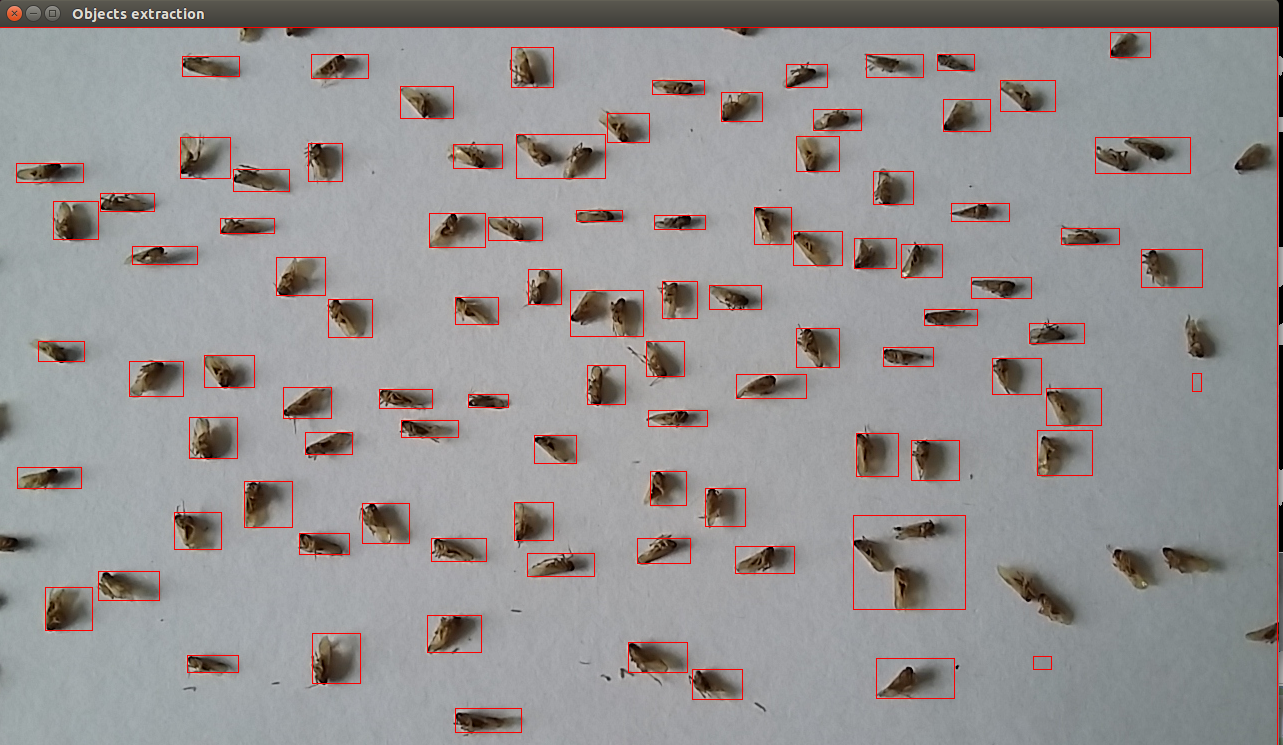
\includegraphics[width=3.6in,height=2.2in]{img/BPHCount.png}
\caption{Brown Planthopper counting (93/106 individuals - accuracy 88\%). The image is taken at 1280x720 resolution with around 50cm distance. In average, each individual has 52.08x30.67 pixels shape and contributes roughly 1063.7 pixels in the image.}
\label{img:BPHCount}
\end{figure}

\item  Moving objects tracking. The approach can be useful in multiple objects tracking. It can accelerate to help tracking 10 to hundreds objects.

\item  Classification. It is able to speed up species classification. For example, it can identify the species of flying birds (figure \ref{img:Birds}).

\begin{figure}[ht]
\centering
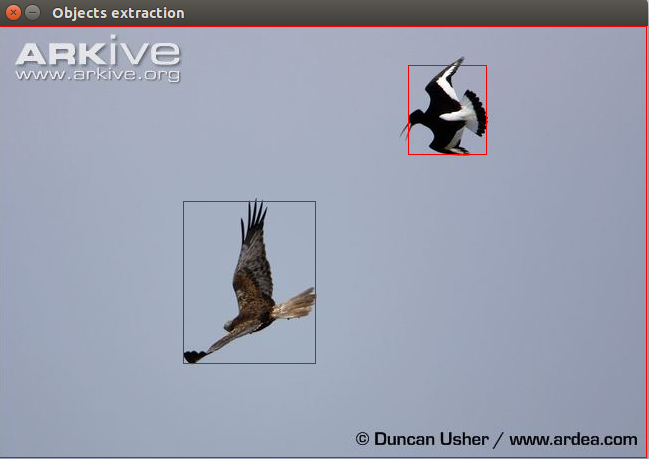
\includegraphics[width=3.6in,height=2.2in]{img/Bird.png}
\caption{Flying bird classification.}
\label{img:Birds}
\end{figure}

\end{itemize}

\subsection {Technical references}

Parallel image processing can be reached thanks to GPUs since the architecture of GPUs is data parallelism \cite{Hillis:1986:DPA:7902.7903} of which varying aspects relate to the memory capacity, the number of processors, feed rates. In most cases, data retrieved from camera is mapped is mapped directly to the GPU and is processed there.

Some examples of parallel vision applications are:
\begin{itemize}
\item A solution inferring  D faces from a single frontal image using automatically extracted 2-D landmarks is proposed in \cite{Choi6163031}. This work uses RANSAC \cite{Fischler:1981:RSC:358669.358692} and Perspective-n-Point (PnP) to estimate the 3D head pose by allowing a large range of poses when the head moves. Experiment shows that this method is able to run in real time thanks to the acceleration of GPU (~15 frames per second - FPS).

\item GPU is also used to speed up the performance in Real Time Image-Based Tracking of 4D Ultrasound Data \cite{Oye2012}. This method allows tracking the location of the probe wrt. anatomy without using external devices. Implementation of the method is carried out in a fast GPU (~8.2FPS) so that the probe can be tracked in real time.

\item Real time performance can be reached by the GPU implementation of a novel model-based method for tracking the six-degrees-of-freedom (6DOF) pose of multiple rigid objects. The method archives the framerate at 40Hz when using  a 500,000 data samples to track 150 objects in 640x480 images. Using an extensive benchmark dataset, the method shows increased performance (in accuracy, robustness, and speed) as compared to state-of-the-art methods. 

\end{itemize}

\subsection {Parallel vision architectures}

The key point of vision applications is the relation between the pixel matrix sensor  and the processing unit. In practice, there are 3 types of cameras as shown in figure \ref{img:Camera}:

\begin{figure}[ht]
\centering
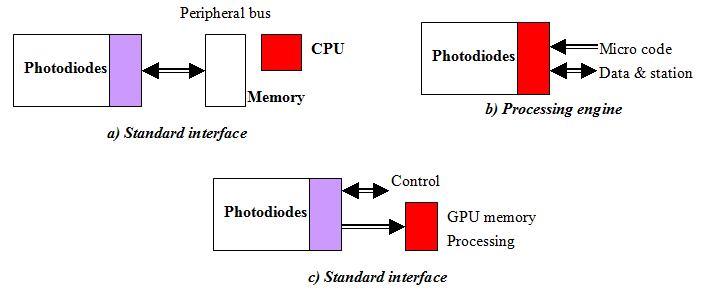
\includegraphics[width=2.8in,height=1.4in]{img/Camera.png}
\caption{3 vision approaches: (a) standard camera with separated vision matrix and processing unit, (b) smart sensor with photodiode matrix and processing on the same chip, (c) camera assembly with DMA between the vision matrix and a graphics processing unit memory (GPU).}
\label{img:Camera}
\end{figure}

Fig. \ref{img:Camera}a  illustrates the architecture of widespread cameras as used in mobile phones, as example. 
They are inexpensive and follow standardization of access interfaces. In principle, a camera has a sensor matrix which is isolated with a processing unit. A micro-controller can control the structure of the image, resolution, acquisition speed in frames per second. This affects the quality of videos relevant to the end user.

Other cameras for industrial controls integrate the processor (a parallel processor) and the sensor array (fig. \ref{img:Camera}b). The analysis can thus be carried out directly into the camera without rendering image format. These cameras can recognize tens of thousands of objects per second, without significant energy expenditure and they also allow the development of machine learning techniques.

Halfway between these two techniques, devices in figure \ref{img:Camera}c) are able to control the acquisition of image segments by sending them directly to a GPU.

What is important in the concept of parallel vision (case 2 and 3) is that
pixels appear in lines, or group of lines,  that are processed as a whole: 
there are no sequential loop over a line, but concurrent processing of several pixels.
This result from the architecture properties and virtualizing the 
processing array.

\subsection {Example algorithm for the counting case}

Figure \ref{img:Count} depicts a workflow useful to count objects such as birds, insects, vessels in an image. 
The context of this workflow is in an insect trap where insects are attracted. 
Periodically, a camera takes an image of the trap and allows to sample  the insect densities locally.

\begin{figure}[ht]
\centering
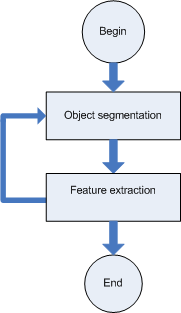
\includegraphics[width=1.2in, height=1.7in]{img/Workflow1.png}
\caption{A workflow for counting object density in an insect trap.}
\label{img:Count}
\end{figure}

\subsubsection {Object segmentation}

Object segmentation from an image input is to detect pixels of an object as 255 (white) while others are  0 (black). The watershed algorithm \cite{DBLP:journals_fuin_RoerdinkM00} is used to implement this task.

The idea is to consider the input image as a topographical surface where pixels with high intensity are peaks and others become valleys. Water is flooded from one valley to another. When water rises, depends on peaks nearby, different valleys tend to merge. Barriers used to prevent the merger may give the segmentation results.

However, it may be oversegmented due to noise and some irregular pixels, thus, a marker based watershed algorithm is used to mark which pixels is are merged and which are not. The idea behind is to label regions that are been sure as foreground with a color and regions that are been sure as background with another color while regions are not been sure anything with 0. Then, the watershed algorithm is applied and the result can be archived.

Figure \ref{img:backgroundmarker} depicts the background and the marker for the result obtained in figure \ref{img:BPHCount}.

\begin{figure}[ht]
\centering
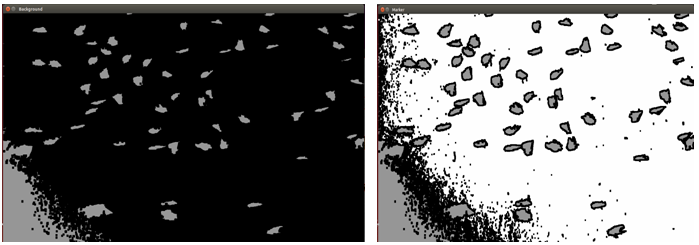
\includegraphics[width=6.2in,height=2.6in]{img/backgroundmarker.png}
\caption{Background (left) and marker (right) for the image in figure \ref{img:BPHCount}.}
\label{img:backgroundmarker}
\end{figure}

The algorithm is shown as follow:

\noindent\rule{16cm}{0.5pt}

\textbf{ALGORITHM}: OBJECT SEGMENTATION

\textbf{INPUT}: source: input image
                  
\textbf{OUTPUT}: result: image output where foreground is white, background is black

\noindent\rule{16cm}{0.5pt}

\lstset{language=C++}
\begin{lstlisting}[basicstyle=\small]

	grayscale = toGrayScale(source);
	binary = threshold(grayscale, t);// binarize image with a threshold t
	erode (binary, foreground); // remove noise and emerge foreground
	// Background is obtained by dilating binary and thresholding
	
	getbackground(binary, background);	
	//marker
	marker = foreground+background;	
	//watershed
	result = doWatershed(source, marker);
}
\end{lstlisting}
\noindent\rule{16cm}{0.5pt}

\subsubsection {Feature extraction} 

The segmentation phasis results in a binary image output used for the second phasis processing. 
Actually, this phasis is to label pixels that belongs to an object as a group and extract features of each group. The connected component labeling algorithm \cite{CCL} is used to implement this phase. 

In the described experiment, color histogram (16 bins for each channel red, green, blue), size (width, height) and area (number of pixels that the object possesses) are considered as object features. Therefore, the feature vector of an object has 51 values.

Due to lack of available data collection, this work assumes that all objects appear in an image belong to a species. 
However, if insect data is collected and managed, it will be possible to create a dataset (e.g tens thousands individuals per species) by using these above features. Thus, the number of objects in an image provides the quantity of necessary insects (e.g result in figure \ref{img:BPHCount}).

{\sl Note : the experiment was coded as a sequential algorithm in advance of a project that will start september 2016}.


\section {Background and perspectives}

Sea shores, and especially archipelagos, represent rich environments where observation is difficult. The paper layout proposes
a set of observation domains, and situation  objectives that could be managed by autonomous networked systems: counting, classifying, tracking.
The first diagnostic is that low power sensing nodes could sample these aspects efficiently under the condition of parallel processing
availability.

Shores are also places where communication infrastructure are likely to be absent. As a result distributed algorithms must manage
knowledge synthesis and transmissions, satellite or plane collection are examples.

We advocate  a design method based on networked smart sensor nodes acting as cyber physical device, 
able to manage interactions between the information system  and the physical aspects, including estimation and simulation of the physical situation. 

A local analysis is supported in each node with the example of  insect/bird counting using watershed and connected component labeling algorithms. It is also shown that local computation can be supported by an architecture for high performance vision suitable to handle object recognition using parallel algorithms. 

Many applications can benefit from approaches similar to integrated vision, as example sound analysis. 

Cyber physical characteristics can also be assessed by the possible control from sensors.
It is known that physical measurements often depend on several basic parameters, and sensors may also affect these measurements. For instance, it is possible to emit light signals of different colors and different intensities to sound environment. It is also possible to rotate the light signals, a camera, a microphone or a speaker. It can be seen that measurements, control devices, recognition, form an indivisible whole which can be classified in the cyber-physic domain.







% \newpage
% \clearpage
%--------Chapter 2 -----------
%\newpage
%\clearpage
%\input{include/chapter2final}
%--------Chapter 3-----------
%\newpage
%\clearpage
%\input{include/chapter3final}
%--------Chapter 4-----------
%\newpage
%\clearpage
%\input{include/chapter4final}
%--------Chapter 5-----------
%\newpage
%\clearpage
%\input{include/chapter5final}
%--------Appendix A-----------
%\newpage
%\clearpage
%\input{include/appendix}

% Referenece by Bibtex
\nocite{*}
\addcontentsline{toc}{chapter}{\numberline{} Bibliography} % For pdf
%\setspecialhdr
\small
\bibliographystyle{plain}
\bibliography{references}

% \newpage
% \clearpage

%End the report
\end{document}
